\chapter{Experiments}

%\section{Notes}

%The fact is the more an agent actually sees the more successful he is in staying alive.

%Too much communication might lead to disorientation of an agent which is subsequently followed by agent's death.

\section{Experimental settings and methodology}

All following experiments are run using a default setup as it is described in this section. Each of the experiments is run on a quadcore \emph{Intel Core i5 with 2,4 GHz and 6 GB RAM}. 
                                                   
Environment is set to be a square matrix with \emph{64 x 64 dimension}. All agents start in the middle of the environment. There are \emph{six kinds of food} which are randomly positioned in the environment and which generate a piece of food each \emph{50 steps}.

Since an environment contains of six food kinds, an agent has six internal variables for each such food kind (see \ref{experiments:singleagent}). By default they are set to 0 and are increased by \emph{0.001 each step} in simulation. When they are equal to 1 (or higher), the agent dies.  

\begin{figure}[h!]
  \centering                                
  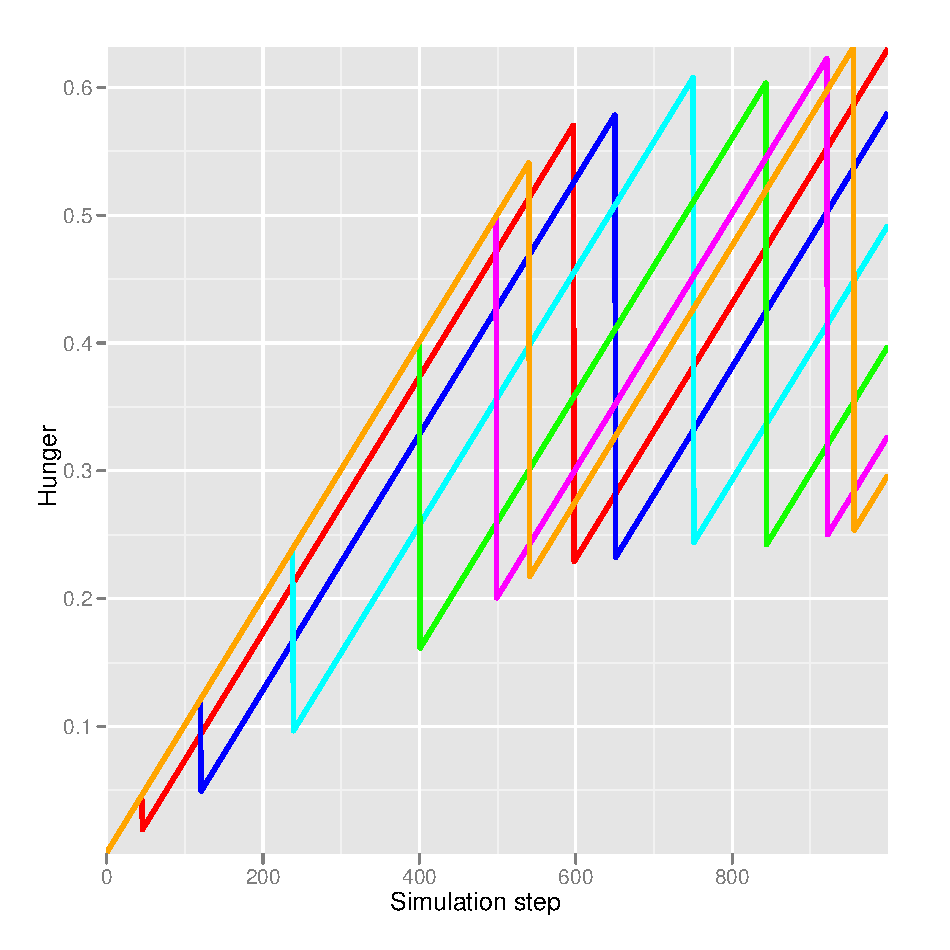
\includegraphics[scale=0.4]{diagrams/experiments/single_agent.eps}    
  \caption{An example of agent's first 1000 steps showing the needs for each kind of food.}
  \label{experiments:singleagent}
\end{figure}



\section{Homogeneus agent set comparision with communication}

In this experiment I will compare avarage life span and efficiency of groups which contains of agents with only single type of memory. Thereby you can see which of the used memory implementation works better in memory homogeneus environment.

What I assume is the \emph{random agents} are about to expire almost immediately as they had no chance to find all the food. While the \emph{PR agents} should approach their goals easily, thereby they will stay alive. Both results of \emph{GNG agent} and \emph{grid agent} are matters of the experiment and I can only expect them not to be worse than \emph{random agent} and not to be better than \emph{PR agent}.     

\clearpage

\subsection{Random agent}   

As for the random agents I assumed that they will immediately pass away without communication. And as you can see in \ref{experiments:random-silent} it happened to be true. 

On the other hand, if I allow them to communicate with each other it might happen they improve their chances. Although they will not last through the entire simulation (see \ref{experiments:gng-grid-pr-random}), the result is that they have managed to slow down [it] (see \ref{experiments:random-start}).

\begin{center}   
  \begin{tabular}{l*{6}{c}r}
  Agent kind        & median & mean & min & max \\
  \hline  
  Random agents with communication     & 1 & 0.875 & 0.406 & 1  \\
  Random agents without communication    & 1 & 1 & 1 & 1  \\
  \end{tabular}                  
\end{center}

%[1] "random median 1 mean 0.874769898839592 min 0.405711205 max 1"
%[1] "random_silent median 1 mean 1 min 1 max 1"

\begin{figure}[h!]
  \centering      
  \subfigure{                   
    \includegraphics[scale=0.35]{diagrams/experiments/random.eps}                                                               
    \label{experiments:random}      
  }  
  \subfigure{                        
    \includegraphics[scale=0.35]{diagrams/experiments/random_silent.eps}       
    \label{experiments:random-silent}
  }
  \caption{Random agent \emph{without communication} fades out quickly.}
\end{figure} 

%\begin{figure}[h!]
%  \centering                    
%  \caption{Random agent with communication manages to survive several thousand steps (see \ref{experiments:random-start}).}
%\end{figure}             

\begin{figure}[h!]
  \centering                                
  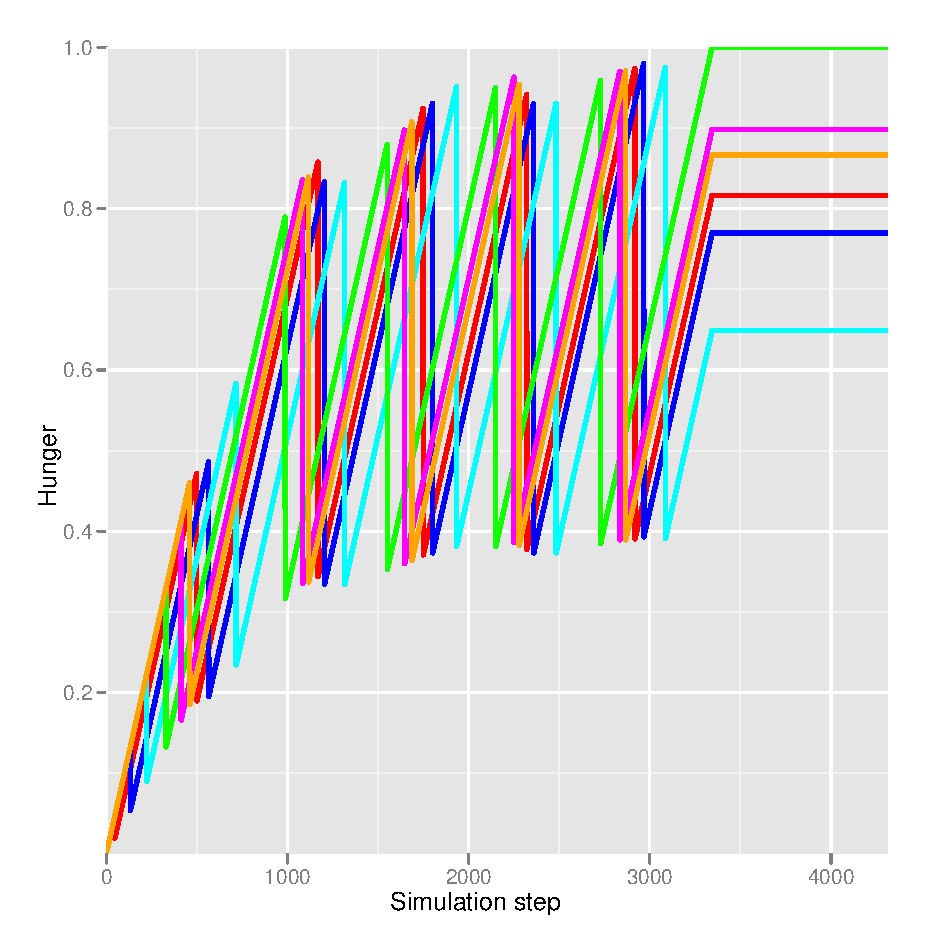
\includegraphics[scale=0.4]{diagrams/experiments/random_start.eps}    
  \caption{A beginning of life of a random agent with communication.}
  \label{experiments:random-start}
\end{figure}        

\clearpage

\subsection{PR agent}

In case of the \emph{pure reactive agents} there is not much to compare between simulation with and without the communication, because the communication is not used since the PR agents see all the environment. So both graphs \ref{experiments:pr} and \ref{experiments:pr-silent} are the same.

\begin{center}   
  \begin{tabular}{l*{6}{c}r}
  Agent kind        & median & mean & min & max \\
  \hline  
  PR agents with communication        & 0.510 & 0.512 & 0.382 & 0.695 \\
  PR agents without communication     & 0.510 & 0.512 & 0.382 & 0.695 \\
  \end{tabular}                  
\end{center}

%[1] "pr median 0.510078733 mean 0.512463510944543 min 0.381653335 max 0.694602152"  
%[1] "pr_silent median 0.510078733 mean 0.512463510944543 min 0.381653335 max 0.694602152"

\begin{figure}[h!]
  \centering       
  \subfigure{                         
    \includegraphics[scale=0.35]{diagrams/experiments/pr.eps} 
    \label{experiments:pr}  
  }
  \subfigure{
    \includegraphics[scale=0.35]{diagrams/experiments/pr_silent.eps}   
    \label{experiments:pr-silent} 
  }
  \caption{PR agent with and without communication.}
\end{figure} 

\clearpage

\subsection{GNG agent}

GNG agents need more information to be able to learn and to survive that is why I do not expect them to deal with it well. In case of a simulation without communication they might end up similarly to random agents, they should do better if they communicate.

\begin{center}   
  \begin{tabular}{l*{6}{c}r}
  Agent kind        & median & mean & min & max \\
  \hline  
  GNG agents with communication        & 0.507 & 0.508 & 0.353 & 0.676W \\
  GNG agents without communication        & 1 & 1 & 1 & 1 \\
  \end{tabular}                  
\end{center}

%[1] "gng median 0.507271498 mean 0.508665935250539 min 0.352669558 max 0.675723953"
%[1] "gng_silent median 1 mean 1 min 1 max 1"

\begin{figure}[h!]
  \centering      
  \subfigure{                          
    \includegraphics[scale=0.35]{diagrams/experiments/gng.eps}     
    \label{experiments:gng}        
  }      
  \subfigure{                                        
    \includegraphics[scale=0.35]{diagrams/experiments/gng_silent.eps}    
    \label{experiments:gng-silent}
  }
  \caption{GNG agent with and without communication.}
\end{figure} 

\clearpage

\subsection{Grid agent}            

I assumed they will do simirarly like GNG agent, i.e. they fail to survive without communication, which assumption ended up to be wrong. Grid agents are able to learn quickly the environment just by moving around randomly and there is the chance that a couple of them survive.

I have run 20 simulations with grid agents to verify the probability of grid agent's learning the environment. As in the standard experiments there were 12 agents and the following values shows the result of the tests:

%8,8,1,9,7,6,8,1,12,3,5,3,4,2,2,4,7,5,6,12

\begin{center}   
  \emph{mean}=5.56, \emph{median}=5.5, \emph{min}=1, \emph{max}=12                 
\end{center}

\begin{center}   
  \begin{tabular}{l*{6}{c}r}
  Agent kind        & median & mean & min & max \\
  \hline  
  Grid agents with communication        & 0.610 & 0.663 & 0.393 & 1 \\
  Grid agents without communication        & 0.495 & 0.680 & 0.338 & 1 \\
  \end{tabular}                  
\end{center}


%[1] "grid median 0.609527062 mean 0.663087118565114 min 0.393369938 max 1"
%[1] "grid_silent median 0.494878372 mean 0.680498955781991 min 0.337940342 max 1"  

\begin{figure}[h!]
  \centering        
  \subfigure{                        
    \includegraphics[scale=0.35]{diagrams/experiments/grid.eps}   
  }
  \subfigure{                                          
    \includegraphics[scale=0.35]{diagrams/experiments/grid_silent.eps}   
  }                                
  \caption{Grid agent with and without communication.}           
  \label{experiments:gng}  
\end{figure} 

\clearpage

\section{Mixed environment}
                        
Second part of the experiments are about environment where different kinds of agents are trying to fulfill their needs. I will observer whether some kind of agents prosper from a presence of other agents or if they are not that successful as they were in a homogeneous environment in previous experiments.
                                                                                
\subsection{GNG+Grid+PR+Random agents}

First I will start with combination of all kinds of agents, whereby since there are those PR agents the others have an advantage of the perfect source of information.  

Results of a simulation with communication follow:
         
\begin{center}   
  \begin{tabular}{l*{6}{c}r}
  Agent kind        & median & mean & min & max \\
  \hline
  GNG agents        & 0.517 & 0.520 & 0.402 & 0.705  \\
  Grid agents       & 0.517 & 0.519 & 0.376 & 0.664  \\   
  PR agents         & 0.513 & 0.513 & 0.380 & 0.644 \\  
  Random agents     & 0.522 & 0.525 & 0.407 & 0.683  \\
  All agents        & 0.517 & 0.519 & 0.376 & 0.705  \\ 
  \end{tabular}                  
\end{center}
       
Results of a simulation without communication follow:
              
\begin{center}
  \begin{tabular}{l*{6}{c}r}
  Agent kind        & median & mean & min & max \\
  \hline
  GNG agents        & 1 & 1 & 1 & 1  \\
  Grid agents       & 0.458 & 0.622 & 0.329 & 1  \\   
  PR agents         & 0.427 & 0.428 & 0.320 & 0.545 \\  
  Random agents     & 1 & 1 & 1 & 1  \\
  All agents        & 1 & 0.762 & 0.320 & 1  \\ 
  \end{tabular}                    
\end{center} 

%[1] "gng-grid-pr-random gng median 0.517498824 mean 0.520457882330892 min 0.401810208 max 0.705358268"
%[1] "gng-grid-pr-random grid median 0.517397617 mean 0.518959058923229 min 0.375598372 max 0.663586088"
%[1] "gng-grid-pr-random pr median 0.51293467 mean 0.51317722590212 min 0.380455353 max 0.644423782"
%[1] "gng-grid-pr-random random median 0.522044497 mean 0.524666185266445 min 0.40689119 max 0.68311006"
%[1] "gng-grid-pr-random all median 0.517392405 mean 0.519315152575945 min 0.375598372 max 0.705358268"

%[1] "gng-grid-pr-random_silent gng median 1 mean 1 min 1 max 1"
%[1] "gng-grid-pr-random_silent grid median 0.45767045 mean 0.621676191740916 min 0.329381465 max 1"
%[1] "gng-grid-pr-random_silent pr median 0.42709512 mean 0.427902891426919 min 0.31951149 max 0.545068625
%[1] "gng-grid-pr-random_silent random median 1 mean 1 min 1 max 1"
%[1] "gng-grid-pr-random_silent all median 1 mean 0.76239074081787 min 0.31951149 max 1"

\begin{figure}[h!]
  \centering        
  \subfigure{                        
    \includegraphics[scale=0.35]{diagrams/experiments/gng-grid-pr-random.eps}    
    \label{experiments:gng-grid-pr-random}
  }     
  \subfigure{
    \includegraphics[scale=0.35]{diagrams/experiments/gng-grid-pr-random_silent.eps}    
    \label{experiments:gng-grid-pr-random-silent}
  }                                                       
  \caption{GNG, grid, PR and random agents together. Owing to PR agents and the communication they all do well.}
\end{figure}
       
\clearpage
                                
\subsection{GNG+Grid+Random agents}

In this experiment I have omitted pure reactive agents and thus left others on their own. For better comparision I have added the difference between values in the current experiment and the previous one (GNG+Grid+PR+Random). I used red colour for a decrease and green colour for an increase, although it is an improvement if they values are lower.         
            
\begin{center}
  \begin{tabular}{l*{6}{c}r}
  Agent kind        & median & mean & min & max \\
  \hline
  GNG agents        & 0.514                   & 0.515                   & 0.367                  & 0.681  \\
                    & \color{red}{-0.003}     & \color{red}{-0.005}     & \color{red}{-0.035}    & \color{red}{-0.024}      \\
  Grid agents       & 0.519                   & 0.521                   & 0.380                  & 0.703   \\   
                    & \color{green}{+0.002}   & \color{green}{+0.003}   & \color{green}{+0.004}  & \color{green}{+0.037} \\
  Random agents     & 0.521                   & 0.523                   & 0.399                  & 0.690   \\
                    & \color{red}{-0.001}     & \color{red}{-0.002}  	& \color{red}{-0.008}    & \color{red}{-0.007}  \\
  All agents        & 0.518                   & 0.520                   & 0.366                  & 0.703  \\
                    & \color{green}{+0.001}   & \color{green}{+0.001}   & \color{red}{-0.001}  &   \color{red}{-0.002}    \\
  \end{tabular}                                
\end{center}

\begin{center} 
  \begin{tabular}{l*{6}{c}r}
  Agent kind        & median & mean & min & max \\
  \hline
  GNG agents        & 1 & 1 & 1 & 1  \\
                    &   \\
  Grid agents       & 1                     & 0.684                 & 0.284                & 1  \\  
                    & \color{green}{+0.542}  & \color{green}{0.062}  & \color{red}{-0.045}  \\
  Random agents     & 1 & 1 & 1 & 1  \\         
                    & \\
  All agents        & 1 & 0.895                 & 0.284 & 1  \\  
                    &   & \color{green}{+0.133}  & \color{red}{-0.036} \\
  \end{tabular}                                        
\end{center}

%[1] "gng-grid-random gng median 0.513585545 mean 0.515161254947844 min 0.366747508 max 0.68104115"
%[1] "gng-grid-random grid median 0.519329297 mean 0.521224015765316 min 0.379762677 max 0.70251225"
%[1] "gng-grid-random random median 0.521283782 mean 0.523338505970543 min 0.399325375 max 0.690103117"
%[1] "gng-grid-random all median 0.518339753 mean 0.519907925561234 min 0.366747508 max 0.70251225"

%[1] "gng-grid-random_silent gng median 1 mean 1 min 1 max 1"
%[1] "gng-grid-random_silent grid median 1 mean 0.684049964170167 min 0.283994157 max 1"
%[1] "gng-grid-random_silent random median 1 mean 1 min 1 max 1"
%[1] "gng-grid-random_silent all median 1 mean 0.894683321390056 min 0.283994157 max 1"

\begin{figure}[h!]
  \centering      
  \subfigure{                          
    \includegraphics[scale=0.35]{diagrams/experiments/gng-grid-random.eps}    
    \label{experiments:gng-grid-random}
  }                                                                              
  \subfigure{                                                  
    \includegraphics[scale=0.35]{diagrams/experiments/gng-grid-random_silent.eps}      
    \label{experiments:gng-grid-random-silent}                                     
  }
  \caption{GNG, grid, PR agents together with and without the communication.}
\end{figure} 
              
\clearpage
                                       
\subsection{GNG+Grid agents}

In this experiment I have observed a simulation with just memory agents in it. Again you can see highlighted differences between new values from this experiment and the values from the previous one (GNG+Grid+Random).


\begin{center} 
  \begin{tabular}{l*{6}{c}r}
  Agent kind        & median & mean & min & max \\
  \hline
  GNG agents        & 0.531                  & 0.533                 & 0.369                 & 0.699  \\  
                    & \color{green}{+0.017}  & \color{green}{+0.018} & \color{green}{+0.002}  & \color{green}{+0.018} \\
  Grid agents       & 0.537                  & 0.538                 & 0.392                & 0.698  \\  
                    & \color{green}{+0.018}  & \color{green}{+0.017} & \color{green}{+0.012}& \color{red}{-0.005}   \\
  All agents        & 0.534                  & 0.535                 & 0.369                 & 0.699  \\
                    & \color{green}{+0.016}  & \color{green}{+0.015}  & \color{red}{+0.003}  & \color{red}{-0.004} 
  \end{tabular}                       
\end{center}

\begin{center}
  \begin{tabular}{l*{6}{c}r}
  Agent kind        & median & mean & min & max \\
  \hline
  GNG agents        & 1 & 1 & 1 & 1  \\   
                    & \\
  Grid agents       & 1 & 0.690                 & 0.282 & 1  \\  
                    &   & \color{green}{+0.006} & \color{red}{-0.002}  \\
  All agents        & 1 & 0.845               & 0.282 & 1  \\
                    &   & \color{red}{-0.05} & \color{red}{-0.002} \\
  \end{tabular}                                 
\end{center}

%[1] "gng-grid gng median 0.530844869 mean 0.532577119282145 min 0.369194478 max 0.699483242"
%[1] "gng-grid grid median 0.537313482 mean 0.53826222964025 min 0.392363958 max 0.698047095"
%[1] "gng-grid all median 0.534081045 mean 0.535419708708437 min 0.369194478 max 0.699483242"

%[1] "gng-grid_silent gng median 1 mean 1 min 1 max 1"
%[1] "gng-grid_silent grid median 1 mean 0.689744413969736 min 0.281647983 max 1"
%[1] "gng-grid_silent all median 1 mean 0.844870337997831 min 0.281647983 max 1"


\begin{figure}[h!]
  \centering          
  \subfigure{                      
    \includegraphics[scale=0.35]{diagrams/experiments/gng-grid.eps}
    \label{experiments:gng-grid}
  }
  \subfigure{                                              
    \includegraphics[scale=0.35]{diagrams/experiments/gng-grid_silent.eps} 
    \label{experiments:gng-grid-silent}  
  }
  \caption{GNG and grid agents together.}
\end{figure}